%  LaTeX support: latex@mdpi.com 
%  In case you need support, please attach all files 
%  that are necessary for compiling as well as the log file, 
%  and specify the details of your LaTeX setup 
%  (which operating system and LaTeX version / tools you are using).

%=================================================================
\documentclass[ijgi,article,submit,moreauthors,pdftex]{Definitions/mdpi} 


%=================================================================
\firstpage{1} 
\makeatletter 
\setcounter{page}{\@firstpage} 
\makeatother
\pubvolume{xx}
\issuenum{1}
\articlenumber{5}
\pubyear{2019}
\copyrightyear{2019}
%\externaleditor{Academic Editor: name}
\history{Received: date; Accepted: date; Published: date}
%\updates{yes} % If there is an update available, un-comment this line

%% MDPI internal command: uncomment if new journal that already uses continuous page numbers 
%\continuouspages{yes}

%------------------------------------------------------------------
% The following line should be uncommented if the LaTeX file is uploaded to arXiv.org
%\pdfoutput=1

%=================================================================
% Add packages and commands here. The following packages are loaded in our class file: fontenc, calc, indentfirst, fancyhdr, graphicx, lastpage, ifthen, lineno, float, amsmath, setspace, enumitem, mathpazo, booktabs, titlesec, etoolbox, amsthm, hyphenat, natbib, hyperref, footmisc, geometry, caption, url, mdframed, tabto, soul, multirow, microtype, tikz

\usepackage{xspace}


%=================================================================
%% Please use the following mathematics environments: Theorem, Lemma, Corollary, Proposition, Characterization, Property, Problem, Example, ExamplesandDefinitions, Hypothesis, Remark, Definition, Notation, Assumption
%% For proofs, please use the proof environment (the amsthm package is loaded by the MDPI class).




\graphicspath{{images/}}

\newcommand{\Astar}{A$^{\!\star}$\xspace}

\newcommand{\e}[1]{\times 10^{#1}}
\newcommand{\fig}{Figure~}
\newcommand{\eq}{Equation~}
\newcommand{\fo}{Formula~}
\newcommand{\sect}{Section~}
\newcommand{\mytable}{Table~}
\newcommand{\chap}{Chapter~}
\newcommand{\figs}{Figures~}
\newcommand{\eqs}{Equations~}
\newcommand{\fos}{Formulas~}
\newcommand{\sects}{Sections~}
\newcommand{\tabs}{Tables~}
\newcommand{\chaps}{Chapters~}


%=================================================================
% Full title of the paper (Capitalized)
\Title{Paralleling Generalization Operations to Support Smooth Zooming:
Case Study of Merging Land-Cover Areas}
%\Title{Merging land-cover areas parallelly 
%to support smooth zooming of web maps}

% Author Orchid ID: enter ID or remove command
\newcommand{\orcidauthorA}{0000-0000-000-000X} % Add \orcidA{} behind the author's name
%\newcommand{\orcidauthorB}{0000-0000-000-000X} % Add \orcidB{} behind the author's name

% Authors, for the paper (add full first names)
\Author{
Firstname Lastname $^{1,\dagger,\ddagger}$\orcidA{}, 
Firstname Lastname $^{1,\ddagger}$ and 
Firstname Lastname $^{2,}$*}

% Authors, for metadata in PDF
\AuthorNames{Firstname Lastname, Firstname Lastname and Firstname Lastname}

% Affiliations / Addresses (Add [1] after \address if there is only one affiliation.)
\address{%
$^{1}$ \quad Affiliation 1; e-mail@e-mail.com\\
$^{2}$ \quad Affiliation 2; e-mail@e-mail.com}

% Contact information of the corresponding author
\corres{Correspondence: e-mail@e-mail.com; Tel.: (optional; include country code; 
if there are multiple corresponding authors, add author initials) +xx-xxxx-xxx-xxxx (F.L.)}

% Current address and/or shared authorship
\firstnote{Current address: Affiliation 3} 
\secondnote{These authors contributed equally to this work.}
% The commands \thirdnote{} till \eighthnote{} are available for further notes

%\simplesumm{} % Simple summary

%\conference{} % An extended version of a conference paper

% Abstract (Do not insert blank lines, i.e. \\) 
\abstract{
%meaning of time.
Land-cover areas are important features on maps.
When users zoom out on digital maps, 
some land-cover areas become too tiny to be seen, 
which result in visual clutters. 
To avoid this problem, 
we merge small areas into their neighbors to form larger areas. 
We define an \emph{event} as merging a small area into a neighbor 
(where the neighbor gradually expands over the small area).
However, because of the given sequence 
in which the events are processed one by one, 
the map users still experience many small shock changes 
(because the merging transition time of their zooming out can be short).
We try to produce smoother changes by paralleling some generalization operations,
which in our case are the merging events.
We define a \emph{step} as a set of merging events happening at the same time.
In our method, a merging step is completely processed 
before the next merging step takes place (all sequential). 
In this way, each event has more time to be observed by users,
resulting in smoother zooming. 
Furthermore, we require that 
all the pairs of areas involved in the merging events of a step 
do not have any common neighbors, 
which makes the merging events independent from each other.
There are two benefits of this independency.
First, it is easy for us to maintain the topology of the map.
Second, users can more easily understand the events 
than merging several areas into a single one.
This paper shows the details of finding and processing parallel events.
Then, this paper compares between the scale transitions of maps generated
based on single-event merging step and parallel-event merging step.
Our original contribution is the proposal of the parallel generalization
maintaining map consistency over scale change. 
%why? how? what? so what?
%%%%
%%%% Alternative abstract
%When users zoom out on digital maps, 
%some land-cover areas become too tiny to be seen, 
%resulting in visual clutters. 
%To avoid this problem, 
%we merge small areas into their neighbors to form larger areas.
%We define an \emph{event} as merging a small area into a neighbor 
%(where the neighbor gradually expands over the small area).
%We define a \emph{step} as a set of merging events happening at the same time.
%A step is completely processed 
%before the next step takes place (all sequential). 
%We produce smooth zooming based on finding parallel events for merging steps,
%where an area participates in at most one event in a step.
%This talk shows the details of finding and processing parallel events.
%Then, this talk compares between the scale transitions of maps generated
%based on single-event step and parallel-event step.
%Our original contribution is the proposal of the parallel merging
%maintaining map consistency over scale transitions. 
}

% Keywords
\keyword{Map generalization, Vario-scale maps, Continuous generalization}



%%%%%%%%%%%%%%%%%%%%%%%%%%%%%%%%%%%%%%%%%%
% Only for the journal Data:
%\dataset{DOI number or link to the deposited data set in cases where the data set is published or set to be published separately. If the data set is submitted and will be published as a supplement to this paper in the journal Data, this field will be filled by the editors of the journal. In this case, please make sure to submit the data set as a supplement when entering your manuscript into our manuscript editorial system.}

%\datasetlicense{license under which the data set is made available (CC0, CC-BY, CC-BY-SA, CC-BY-NC, etc.)}



%\setcounter{secnumdepth}{4}
%%%%%%%%%%%%%%%%%%%%%%%%%%%%%%%%%%%%%%%%%%
\begin{document}
%%%%%%%%%%%%%%%%%%%%%%%%%%%%%%%%%%%%%%%%%%



\section{Introduction}


When map users are reading digital maps,
they expect different levels of detail (LoDs) depending on scale.
For example, they may want to see individual buildings when zooming in
and see built-up areas when zooming out.
That is why geographical information is dependent on the scale
\citep{Muller1995Generalization,Weibel1997}. 
In order to prepare map data for different scales,
map generalization is employed to generate coarser data 
for maps at smaller scales,
from a detailed map.
A lot of research has been devoted to map generalization.
\citet{Mackaness2017Generalization} gave a taxonomy of 
generalization algorithms, 
including selection, simplification, aggregation, and so on.
Often, a multi-representation database (MRDB) is utilized to store
maps at different scales and to send proper data to clients on request
\citep[\eg][]{Hampe2004multiple}.
However, large discrete changes between different map representations
may confuse users,
so continuous map generalization (CMG) is needed to
provide smooth scale zoom.
Algorithms of CMG have been proposed 
to morph raster maps
\citep[\eg][]{Pantazis2009a,Pantazis2009b}, 
to morph polylines
\citep[\eg][]{Noellenburg2008,Peng2013LSA,Deng2015,Li2017Annealing},
to generalize buildings
\citep[\eg][]{Li2017_Building,Peng2017Building,Touya2017Progressive},
to transform road networks
\citep[\eg][]{Suba2016Road,Chimani2014Eat},
and to transform administrative boundaries
\citep[\eg][]{Peng2016Admin}.
%Indeed, there are already many algorithms 
%for continuous map generalization.
%To adapt them into a web environment still needs a lot of effort.
%This paper contributes to merging land-cover areas 
%in a web environment. 


Land-cover areas are important features on maps. 
When users zoom out,
some land-cover areas become too tiny to be seen,
which result in visual clutter.
The clutter can be avoided by merging those tiny areas 
with their neighbors.
For example, \citet{haunert2008f} developed a method based on
mixed-integer programming to merge land-cover areas
for a map at a certain scale.
However, if zooming is realized by switching between
some levels of map representations, 
large and discrete changes usually happen
(e.g., from \fig\ref{fig:intro}a to \fig\ref{fig:intro}b), 
which is difficult for map users to understand.
To provide small changes, 
\citet{vanOosterom2005} proposed 
the topological Generalized Area Partitioning (tGAP) tree,
where in each step a single area is merged into
its most compatible neighbor 
(see \fig\ref{fig:intro}c--g).
Further, a space-scale cube (SSC) can be built so that 
map users can view the gradual transition of the merge operation
by slicing the SSC \citep[see][]{Meijers2020Web}.
This gradual strategy apparently allows users 
to follow the zooming more easily.


\begin{figure}[tb]
\centering
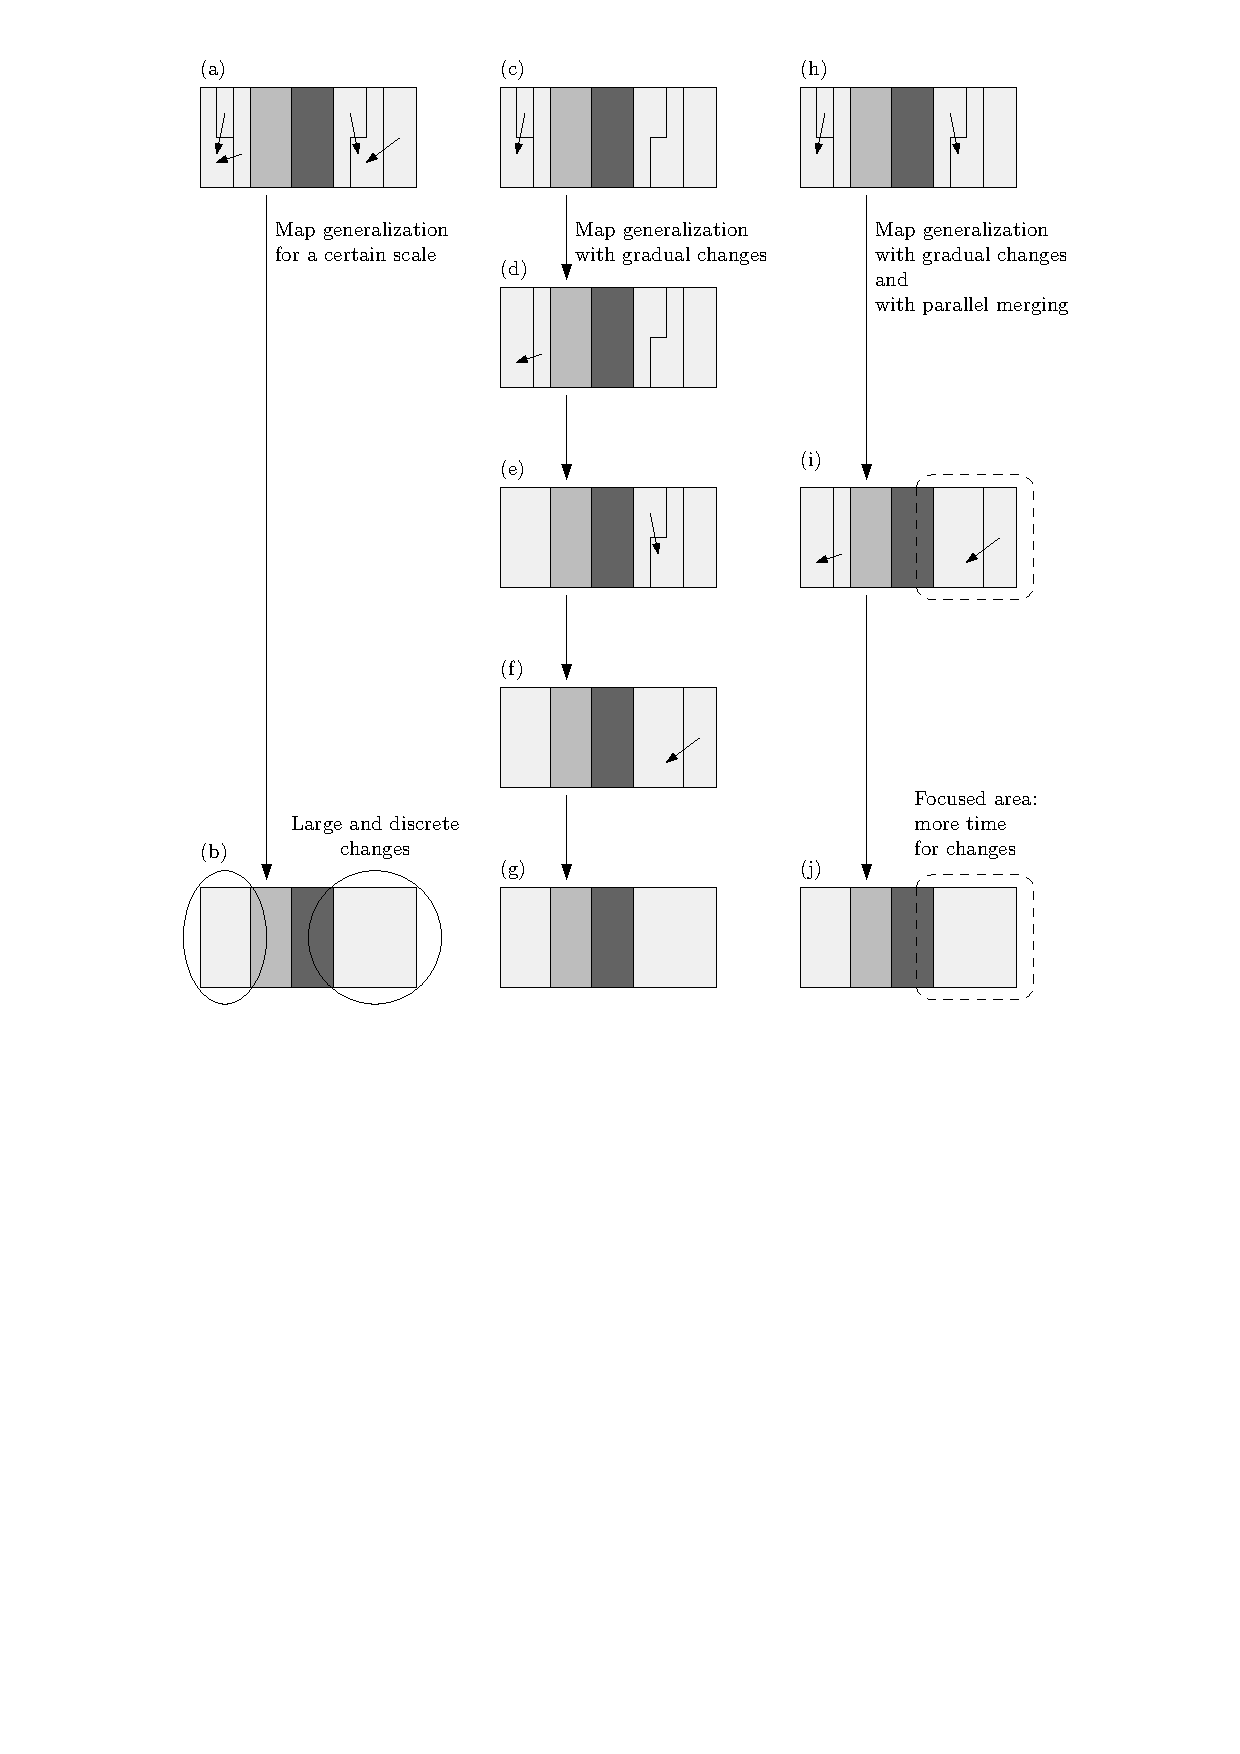
\includegraphics[page=1]{introduction}
\caption{A comparison of traditional map generalization (a--b),
map generalization with gradual changes (c--g),
and map generalization with parallel merging (h--j).
The ellipses show the places where large and discrete changes happen.
The dashed polygons show the place where a user may focus;
in the place, the user has twice of the time to perceive the merging
comparing to the merging of figures e--g.
Each arrow indicates that an area will be merged into another one. 
}
\label{fig:intro}
\end{figure}

When users zoom on maps, 
they do not want to wait for too long 
to see the desired level.
On a real map, however, 
there are way too many pairs of areas to merge 
when users are zooming out.
If the pairs are processed one by one 
(e.g., \fig\ref{fig:intro}c--f),
then the time interval for each merging operation has to be very short.
For example, a user may get the impression of
a direct change from \fig\ref{fig:intro}e to \fig\ref{fig:intro}g
(without the intermediate state of \fig\ref{fig:intro}f)
even when the three areas on the right-hand side of \fig\ref{fig:intro}e
are merged gradually.
To provide users with more gradual impression, 
we parallel the merging operations
(see \fig\ref{fig:intro}h--j).
If we select some of the merging operations
fairly evenly distributed on the whole map 
(there may be only a small number of merging operations 
happening on the screen),
then the changes are easy for users to understand
because these changes now have more time to take place.
For example, in the focused area, there is only one merging operation 
from \fig\ref{fig:intro}i to \fig\ref{fig:intro}j
while there are two merging operations  
from \fig\ref{fig:intro}e to \fig\ref{fig:intro}g;
a user has twice of the time to perceive the changes of the former,
comparing to the latter.

This paper is organized as follows.
\sect\ref{sec:realted_work} reviews some related work.
Our methodology is presented in \sect\ref{sec:methodology}.
We show a case study in \sect\ref{sec:case_study}.
Finally, \sect\ref{sec:concluding_remarks} draws our conclusion
and indicate our future work.





 
\section{Related Work}
\label{sec:realted_work}

\citet{vanOosterom2005} proposed a greedy algorithm 
to merge land-cover areas one by one.
In each iteration, that algorithm takes the least important area and 
merges it into the most compatible neighbor.
The importance of an area is defined 
based on both the size and the type of the area.
The compatibility between a pair of areas is defined based on 
both the length of the common boundary and the similarity of the types 
of the pair of areas. 
\citet[\chap2]{Peng2019Thesis} tried to find an optimal sequence 
to merge land-cover areas
based on the \Astar algorithm or an integer linear program.
A comparison to a greedy algorithm showed that 
the \Astar algorithm improves the quality of the merging sequences
in the sense of the type changes and the compactnesses of the areas.
\citet{vanOosterom2014Support} pointed out that sequentially merging
land-cover areas may result in a suboptimal smooth-zoom effect.
To provide better visualization, they suggested that
the merging operations should be paralleled.
Then, one question is how many operations 
should be paralleled for a given scale.
\citet{Thiemann2018LandCover} proposed a chain of operators 
to generalize a land-cover map.
In the chain of processing land-cover polygons, 
they integrated cleaning, dissolving, splitting, aggregating, reclassifying, and simplifying. 


\citet{Meijers2020Web} explained the principles of 
implementing a web map of land-cover areas.
First, they generated an SSC, 
where an area on map becomes a polyhedron in the SSC.
They used the SSC because 
they wanted the web map to support smooth zoom
\citep[see][]{vanOosterom2014Support}.
Second, they showed how to slice the SSC 
to output a web map at a given scale.
The slicing is based on the GPU at the client side.
Third, they made chunks of the SSC 
so that they were able to send only the data of the place
where a map user was reading.
\citet{Suba2014Merge} proposed three methods 
to merge a pair of areas in a gradual manner, 
which are the ``Single flat plane'', the ``Zipper'', and the ``Eater''.
Basically, the \emph{winner} gradually expands over the \emph{loser}.
We will use the ``Eater'' because it works for all kinds of polygons 
while the other two methods have limitation 
in terms of the type of a polygon.
For example, the two other methods do not work for some concave polygons.
\citet{Suba2016Road} continuously generalized a planar map of road network.
In each step, they process the least important face.
Taking into account the condition of the face,
they put it back with higher importance, collapse it, 
or merge it into an adjacent face.
In addition to the generalization, 
they also observed the number of faces,
the area of faces, the number of road faces, the number of road edges,
and the number of operations (merge and split) 
when the scale of the map is decreasing.
These statistics can be good indications 
for (continuous) map generalization.
\citet{Huang2016Webmap} pointed out that
the effort of implementing online maps 
had been spent mainly on preparing data on the server side.
They studied the communication of map data 
between the server side and the client side.
They proposed different strategies of assigning 
the work of handling map data
according to the machine abilities of the clients.

\citet{Huang2017Matrix} utilized a matrix to guide 
both pruning rivers and removing vertices for a river network, 
where the rows and the columns respectively represent
the rivers and the vertices.
According to the matrix, 
they were able to decide which rivers and vertices 
should be remained for a given scale.
To this purpose, they proposed a method 
to compute how many rivers and vertices 
should be kept according to that given scale.






%\citet{Thiemann2018LandCover}
%\citet{Dumont2020MultiScale}
%\citet{Meijers2015Parallel}

%

\section{Methodology}
\label{sec:methodology}

%UML?
%Flowchart of the framework?

%\subsection{Smooth Merging}
%\label{sec:smooth_merging}

In order to provide smooth zooming of merging
so that map users easily understand the changes,
we merge by gradually expanding an area over another area
(see \fig\ref{fig:smooth_merging}).
This expansion is based on slicing the space-scale cube shown in
\fig\ref{fig:smooth_merging_ssc}.
For example, \figs\ref{fig:smooth_merging}a,
\ref{fig:smooth_merging}b, and \ref{fig:smooth_merging}c
are respectively obtained from slicing the cube 
at the bottom, the middle, and the top.
The details of slicing a cube can be found in \citet{Meijers2020Web}.
The cube of \fig\ref{fig:smooth_merging_ssc} was built 
based on the \emph{Eater} of \citet{Suba2014Merge}.
The Eater was used because it provides a solution 
for an area with any kind of shape, which is more robust than
\emph{Single flat plane} and \emph{Zipper} \citep{Suba2014Merge}.
Note that the common boundary of the two areas disappears
very shortly after the expansion starts;
the common boundary exists only in \fig\ref{fig:smooth_merging}a but not in
\fig\ref{fig:smooth_merging}b,
\fig\ref{fig:smooth_merging}c, or
\fig\ref{fig:smooth_merging}d.


\begin{figure}[tb]
\centering
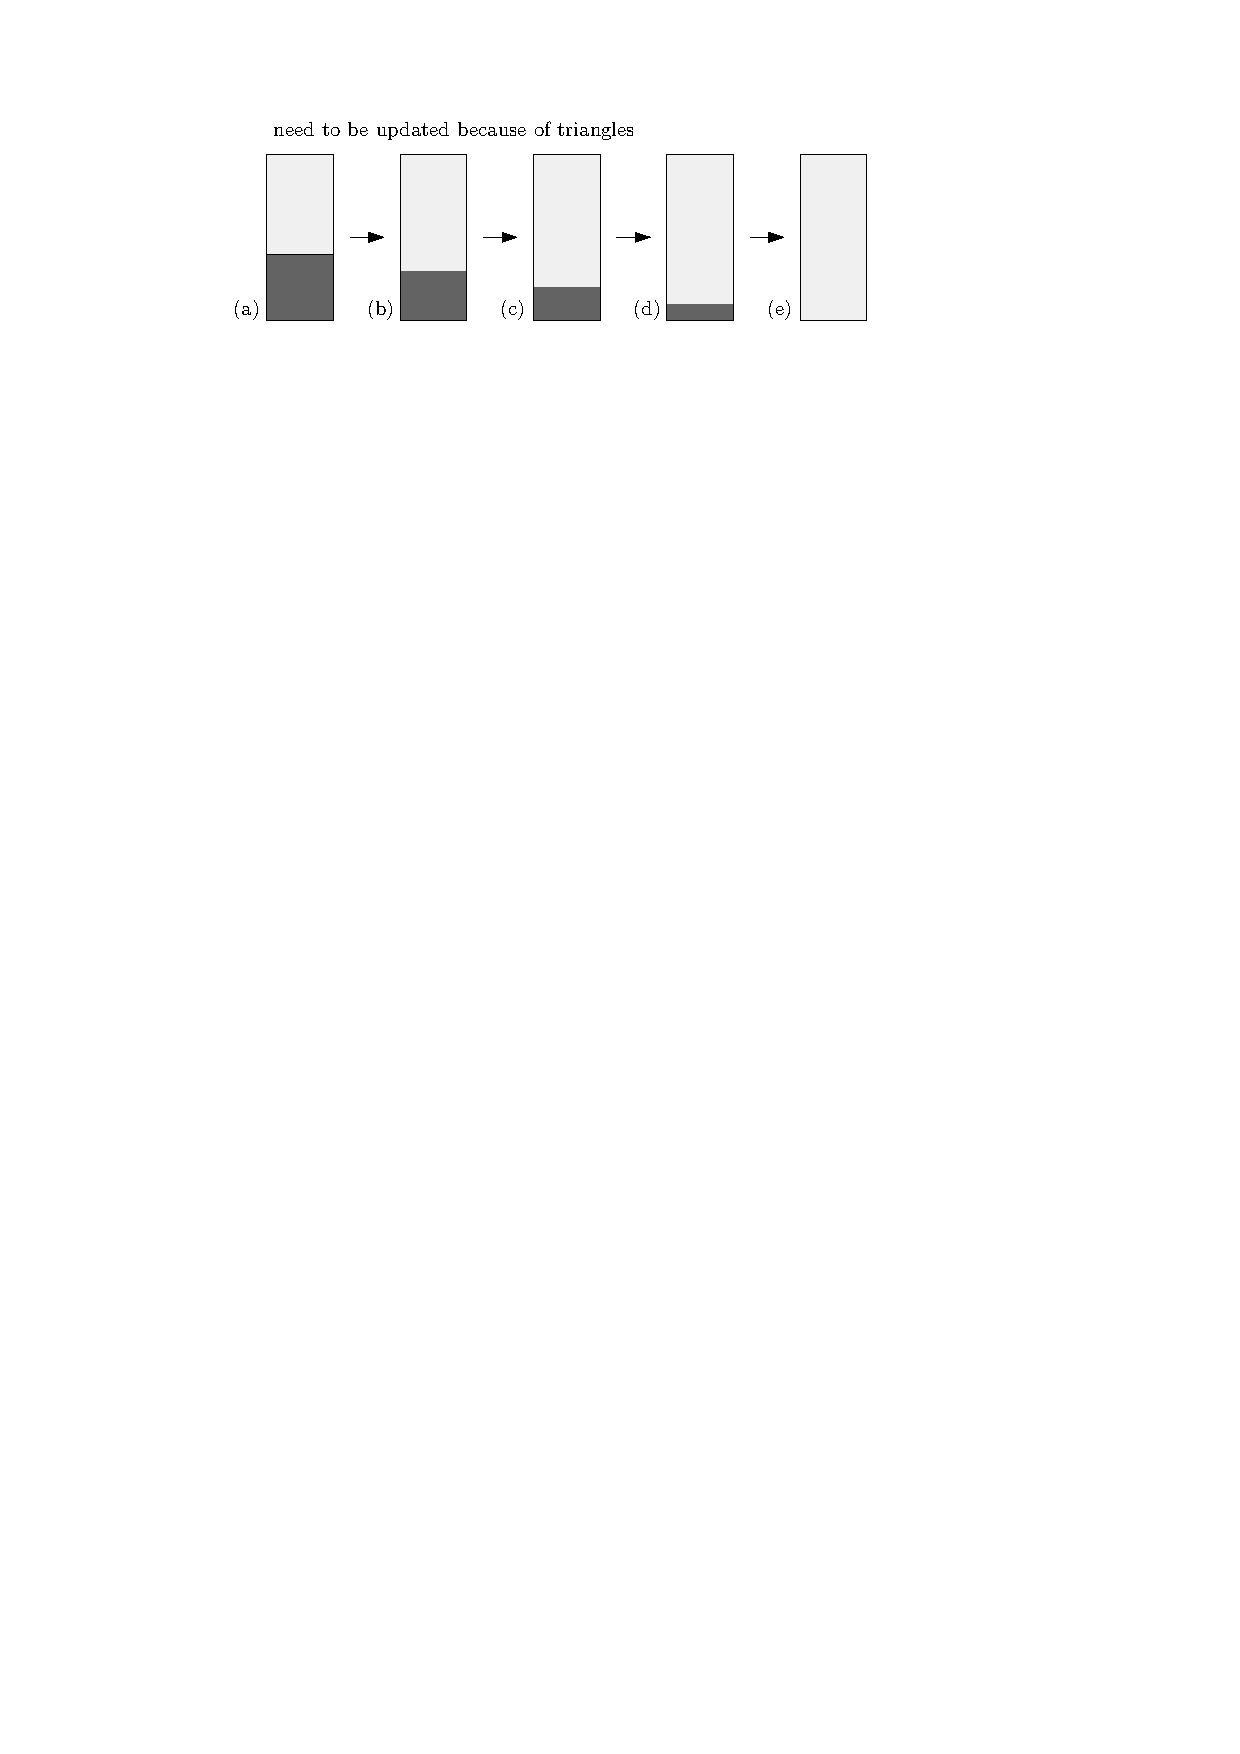
\includegraphics[page=1]{smooth_merging}
\caption{A smooth way of merging two areas,
    where the larger area gradually expands over the smaller one.}
\label{fig:smooth_merging}
%
\vspace{6mm}
%
\centering
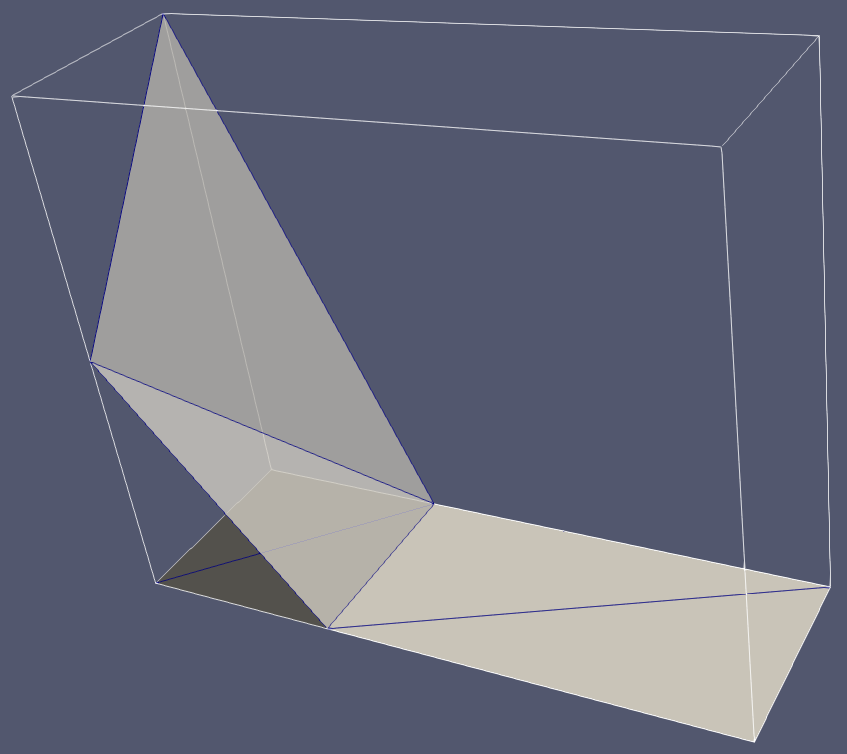
\includegraphics[scale=0.15]{smooth_merging_ssc}
\caption{The space-scale cube for the merging 
    of \fig\ref{fig:smooth_merging}.
    This figure is made by visualizing the content of an obj file in 
    ParaView 5.6.0.}
\label{fig:smooth_merging_ssc}
\end{figure}




We define an \emph{event} as a single generalization operation, 
such as merging a small area into a neighbor.
For example, \fig\ref{fig:event_and_step}b is obtained from 
\fig\ref{fig:event_and_step}a by processing one merging event,
where the dashed polygon marks the new area from the merging.
Similarly, \fig\ref{fig:event_and_step}c is obtained from 
\fig\ref{fig:event_and_step}a by processing two merging events.
We define a \emph{step} as 
a set of events happening at the same time.
For example, 
\fig\ref{fig:event_and_step}b is obtained from 
\fig\ref{fig:event_and_step}a by processing merging step with one event.
\fig\ref{fig:event_and_step}d is obtained from 
\fig\ref{fig:event_and_step}c by processing merging step with two events.
In our method, a merging step is completely processed 
before the next step takes place (all sequential). 

\begin{figure}[tb]
\centering
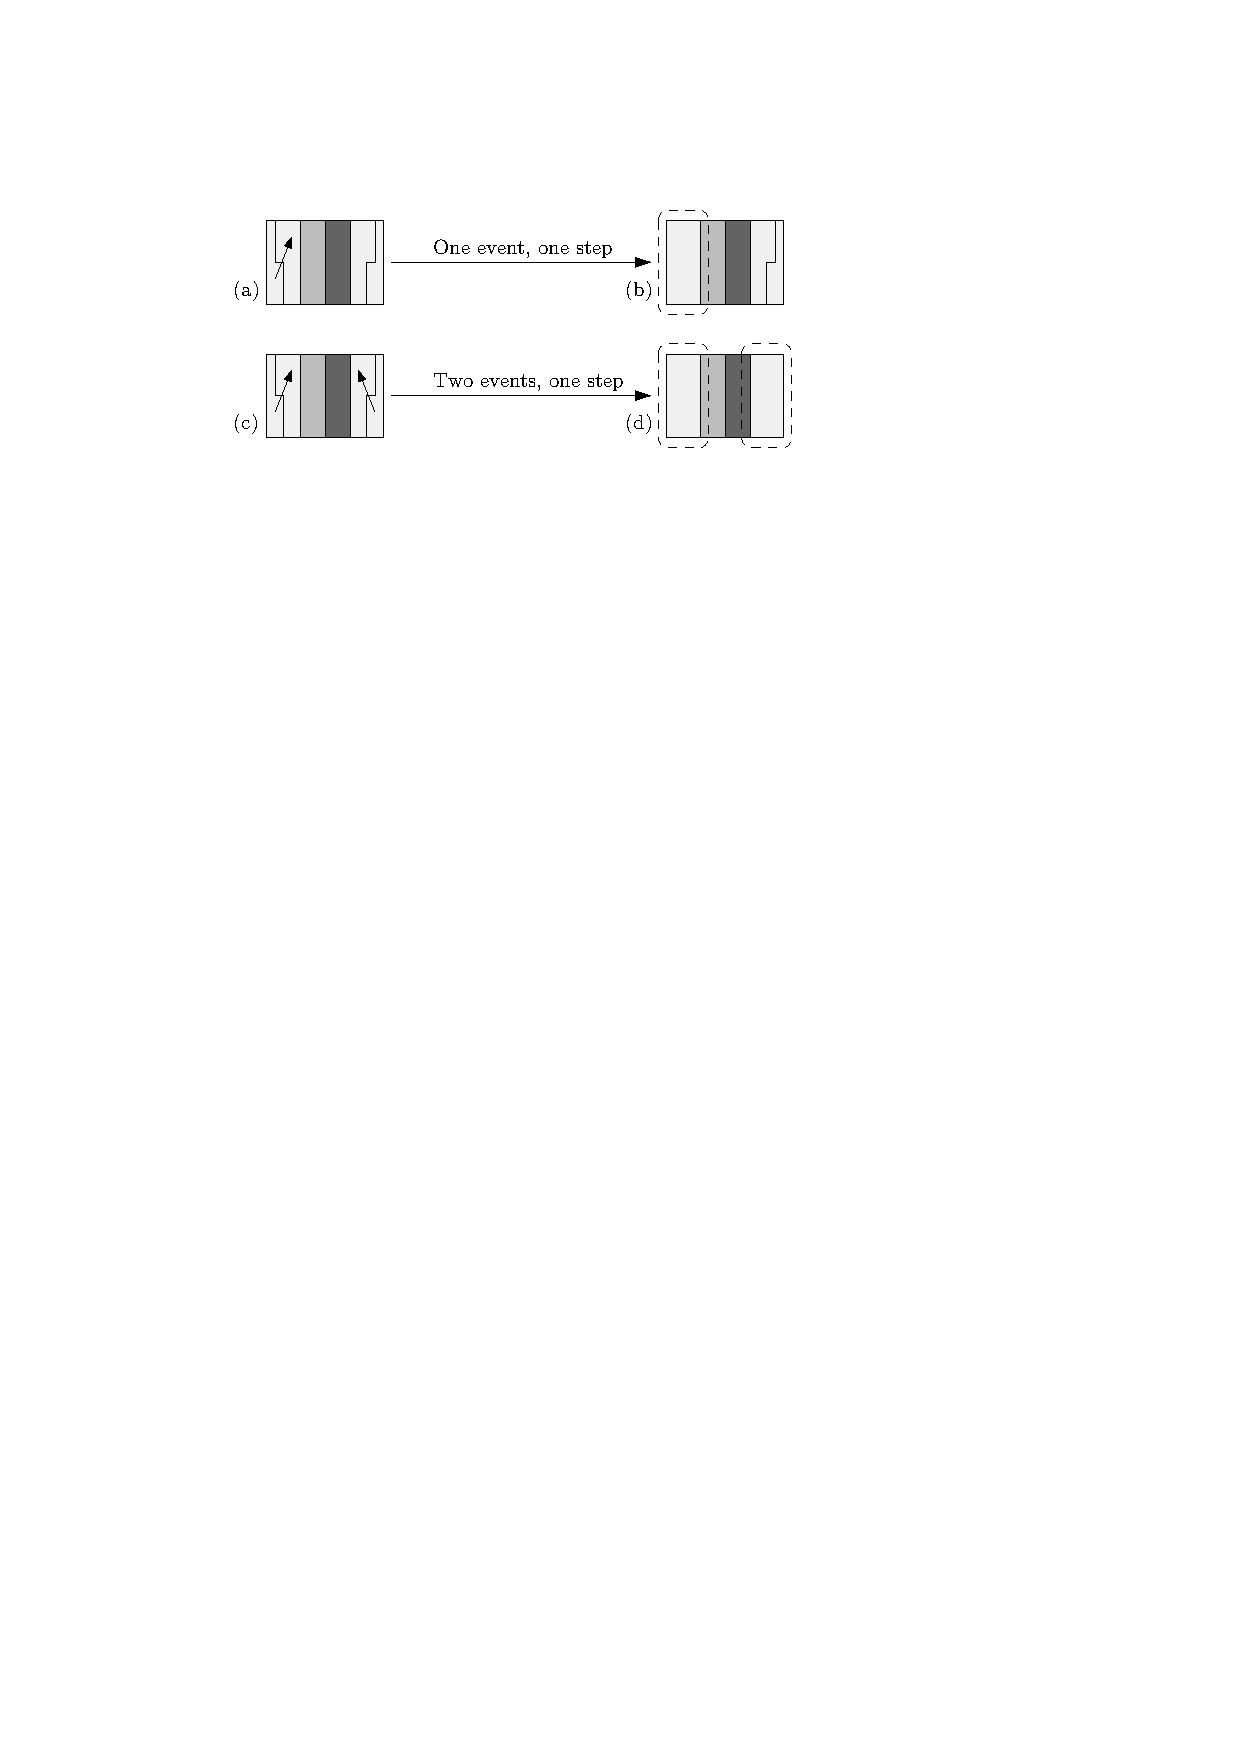
\includegraphics[page=1]{greedy_algorithm}
\caption{Illustration of the merging event and the merging step. 
Each path shows a merging step. 
A merging step consists of one or more merging events.}
\label{fig:event_and_step}
\end{figure}


We require that 
the land-cover areas involved in different merging events of a step 
must not be neighbors, 
which makes the merging events independent from each other.
There are two benefits of this independency.
First, it is easy to maintain the topology of the map.
When a pair of areas have been merged, 
we must update the common boundaries with the adjacent areas.
If an adjacent area is involved in another merging event,
then it is complicated to update the common boundaries 
for the two merging events.
Second, users can understand the events more easily 
than merging several areas into a single one,
where the latter is a traditional way of merging.
In order to realize the requirement, 
we block the neighbors of the areas selected for merging events.
In the following, we show a greedy algorithm 
to find the merging events for each step.


\subsection{A Greedy Algorithm}
\label{sec:greedy_algo}

In the greedy algorithm, we need to obtain the most compatible neighbor 
for a given area.
There are many ways of defining the most compatible neighbor.
For example, \citet{Cheng2006} proposed three ways, i.e.,
the neighbor has the largest size, 
shares longest boundary with the least important area,
or is closest to the least important area in land-cover type. 
\citet{Peng2017AStar} proposed that 
the neighbor should have a close land-cover type
to the least important area
and the combination of the two areas should be compact;
they defined the type distance based on a binary tree
according to the code of each land-cover type.
We currently consider the most compatible neighbor
as the one shares the longest common boundary with the smallest area.

\fig\ref{fig:greedy_framework} shows the framework of our greedy algorithm.
The process starts with state~$s=0$ and a land-cover map.
The parallel parameter~$r_\mathrm{parallel} \in [0,1)$ has to be input.
This parameter specifies the proportion of land-cover areas that
we expect to merge parallel.
Expression~$|M_s|$ denotes the number of areas of the map at state~$s$.
If there are more than one land-cover area ($|M_s|>1$),
then we can start to find merging events.
We first compute the number of areas that we expect to merge by
\begin{equation}
\label{eq:n_expect}
n_\mathrm{expect} =
\lceil r_\mathrm{parallel} \cdot |M_s| \rceil,
\end{equation}
where the ceiling function is used so that 
there holds~$n_\mathrm{expect}\ge 1$.
However, we cannot always merge~$n_\mathrm{expect}$ areas
because some areas may be blocked as explained before
(also see \fig\ref{fig:blocked_polygons}).
Therefore, variable~$n_\mathrm{event}$ is used
to represent the number of events that we have found. 


\begin{figure}[tb]
\centering
\includegraphics[page=2]{greedy_algorithm}
\caption{The flowchart of our greedy algorithm.
}
\label{fig:greedy_framework}
\end{figure}


\begin{figure}[tb]
\centering
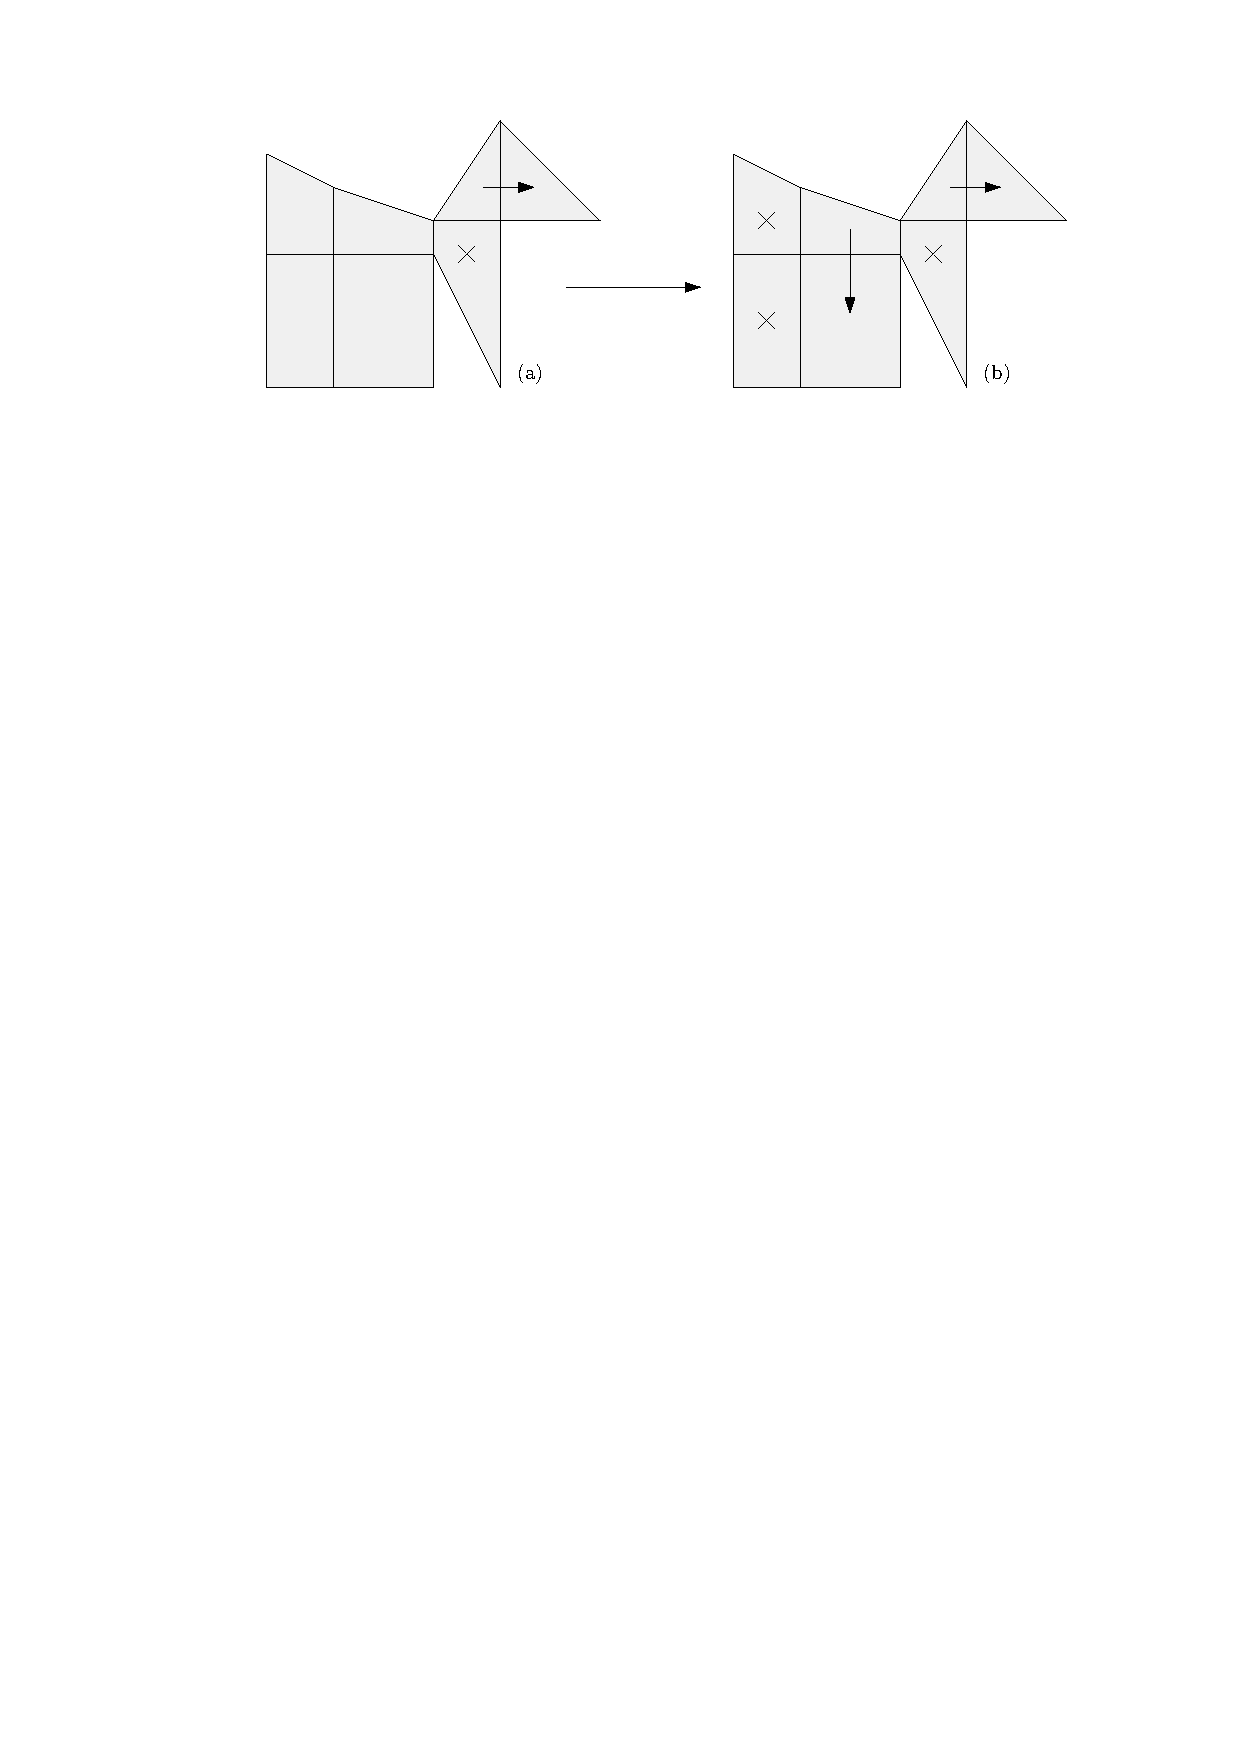
\includegraphics[]{blocked_polygons}
\caption{(a) From all the free areas,
	the least important one is selected to merge into
	its most compatible neighbor (the arrow indicates the merging).
	Then the surrounding areas are blocked (marked by the cross).
	(b) In order to find parallel merging events, 
	the least important area from the remaining free areas
	is selected to merge with the most compatible neighbor
	(the arrow indicates the merging),
	and the surrounding areas are blocked.
}
\label{fig:blocked_polygons}
\end{figure}

If we have not found $n_\mathrm{expect}$ events 
and there are still free areas,
then the least important area~$a_\mathrm{least}$ is selected
from the set of free areas.
An area is \emph{free} if 
it is not involved in an event and is not blocked.
Then the most compatible neighbor~$a_\mathrm{nbr}$ 
of~$a_\mathrm{least}$ is found.
If area~$a_\mathrm{nbr}$ is also free, 
then we form an event for areas~$a_\mathrm{least}$ and~$a_\mathrm{nbr}$,
and increase variable~$n_\mathrm{event}$ by 1.
We also block other neighbors of $a_\mathrm{least}$ and $a_\mathrm{nbr}$
(see \fig\ref{fig:blocked_polygons}a).
Then, we continue to find more merging events
(see \fig\ref{fig:blocked_polygons}b).
If area~$a_\mathrm{nbr}$ is not free,
we block $a_\mathrm{least}$ for now
so that $a_\mathrm{least}$ and $a_\mathrm{nbr}$ 
may merge in the next step.

If we have found $n_\mathrm{expect}$ events 
or there is no free area anymore,
then finding merging events of the step finishes.
Consequently, we merge each pair of the areas of all the events,
free all the blocked areas,
increase state~$s$ by value of~$n_\mathrm{event}$,
and create map~$M_s$ of the new areas and the freed areas.
Then, finding merging events for the next step starts.
This finding completes until there is only one area left on the map.
The merging events will be stored as records in tGAP tables
\citep[see][\p159]{Meijers2011Thesis}.
\fig\ref{fig:sequence_greedy} shows a sequence of merging steps
obtained by our greedy algorithm.

\begin{figure}[tb]
\centering
\includegraphics[page=2]{blocked_polygons}
\caption{A sequence of merging steps obtained by our greedy algorithm,
	where parallel parameter~$r_\mathrm{parallel}$ is set to $0.3$.
	Each arrow in a subfigure indicates a merging event.
}
\label{fig:sequence_greedy}
\end{figure}




\subsection{Integrating the parallel events into the tGAP}

\citet[\p159]{Meijers2011Thesis} designed tables 
to record the information of
faces, edges, and face hierarchy, 
which together form a tGAP.
Take the face table as an example,
it contains columns \emph{face\_id}, 
\emph{imp\_low}, \emph{imp\_high}, \emph{imp\_own},
\emph{feature\_class\_id}, \emph{area}, and \emph{bbox}.
We add columns \emph{state\_start} and \emph{state\_end} into the table 
so that it is easy to see when a face should appear or disappear 
(see \tbls\ref{tbl:face_tgap} and~\ref{tbl:face_tgap_parallel},
where some columns are hidden).
That is, a face should appear
when the merging arrives at the state\_start value,
and the face should disappear
when the merging arrives at the state\_end value.
When switching from single-event merging 
(sequence~I of \fig\ref{fig:face_tgap})
to parallel merging (sequence~II of \fig\ref{fig:face_tgap}),
we observe that the state\_end values of faces~1 and~2 are changed from~1 to~2
(see \tbl\ref{tbl:face_tgap_parallel}, the new values are underlined).
Also, the state\_start value of faces~6 is changed from~1 to~2
(see \tbl\ref{tbl:face_tgap_parallel}).
The columns and records of both the edge table and the face-hierarchy table 
will be changed accordingly.


\subsection{Integrating the parallel events into the SSC}

Before merging a pair of areas by expanding one over the other one,
we must know when to start the expansion.
This information is necessary for building the SSC.
A simple way is to add a column, say, \emph{state\_expand} 
into the face table during generating the tGAP.
Then, the time of starting expansion can be recorded into the column.
However, we would like to keep as few columns as possible
so that the table is easy to read.
As a result, we compute state\_expand values on the fly 
when building the SSC.

By definition, parallel events of a merging step happen at the same time.
In other words, the faces involved in those parallel events have 
the same state\_expand value ($s_\mathrm{expand}$) and 
the same state\_end value ($s_\mathrm{high}$).
The reverse is also true.
If some faces have the same state\_end value,
then the faces are involved in the parallel events of the same step.
The reason is that the mergings of these faces will finish at $s_\mathrm{high}$,
and no merging will start earlier or later than $s_\mathrm{expand}$
because we required that the next step starts only when the current step stops.
As an event involves two faces,
the number of events finishing at state~$s_\mathrm{end}$ can be calculated by
\begin{equation}
\label{eq:n_event_state}
n_\mathrm{event} (s_\mathrm{end}) = 
\frac{\sum\limits_{s \in S_\mathrm{end}} [s=s_\mathrm{end}]}{2},
\end{equation}
where notation~$S_\mathrm{end}$ denotes the set of state\_end values,
and expression~$[s=s_\mathrm{end}]$ returns~$1$ if the two values are equal 
and returns~$0$ otherwise.
The state to start the merging animation is
\begin{equation}
\label{eq:s_expand_state}
s_\mathrm{expand} (s_\mathrm{end}) = s_\mathrm{end} - n_\mathrm{event} (s_\mathrm{end}).
\end{equation}
Take the values in \tbl\ref{tbl:face_tgap_parallel} for example,
we have~$S_\mathrm{high} = \{2, 2, 3, 2, 2, 4, 3, 4, 5\}$, 
$n_\mathrm{event} (2) = 2$, and~$s_\mathrm{expand} (2) = 0$.
Therefore, the merging expansions of faces~1, 2, 4, and 5 
should take place from state~$0$ to state~$2$,
which can be observed from the two tilted faces above the two pink faces 
in \fig\ref{fig:ssc_parallel}.
In merging sequence~I, the expansion of faces 1 and 2 
takes place from state~$0$ to state~$1$
(see the tilted face above the pink face on the left-hand side of \fig\ref{fig:ssc_single}),
and the the expansion of faces 3 and 4
takes place from state~$1$ to state~$2$
(see the tilted face above the pink face on the right-hand side of \fig\ref{fig:ssc_single}).
As a result, the expansion duration of faces 1 and 2 of sequence~II
is twice as that of sequence~II;
the animation with parallel events is easier for a map user to perceive. 


%According to \tbl\ref{tbl:face_tgap}, 
%face~1 and face~2 are merged from state~0 to state~1,
%which is before the merging of face~5 and face~6 from state~1 to state~2.
%According to \tbl\ref{tbl:face_tgap_parallel}, 
%the merging of face~1 and face~2 and the merging of face~5 and face~6
%happen parallelly from state~0 to state~2.
%
%Then, the space-scale cube will be built 
%according to the records of \tbl\ref{tbl:face_tgap_parallel}.


\begin{figure}[tb]
\centering
\includegraphics[page=3]{greedy_algorithm}
\caption{Merging one pair of areas in each step (sequence~I), 
    and merging two pairs of areas parallelly (sequence~II).}
\label{fig:face_tgap}
\vspace{6mm} %for some reason, the space below the caption is not enough
%
%
%
\captionsetup*{type=table} %*: suppress warning "The caption type was already set to figure"
\parbox{.49\linewidth}{
\caption{Some columns of the face table of merging sequence~I, 
    shown in \fig\ref{fig:face_tgap}.}
\label{tbl:face_tgap}
\centering
\begin{tabular}{ccc}
\hline
face\_id &   state\_start   & state\_end    \\ \hline
1       &     0         &     1          \\
2       &     0         &     1          \\
3       &     0         &     3          \\ 
4       &     0         &     2          \\
5       &     0         &     2          \\
6       &     1         &     4          \\         
7       &     2         &     3          \\
8       &     3         &     4          \\ 
9       &     4         &     5          \\ \hline
\end{tabular}
}
%
%
\parbox{.49\linewidth}{
\caption{Some columns of the face table of merging sequence~II, 
    shown in \fig\ref{fig:face_tgap}.}
\label{tbl:face_tgap_parallel}
\centering
\begin{tabular}{ccc} %\underbar{2}
\hline
face\_id &   state\_start & state\_end    \\ \hline
1       &     0         & \underbar{2}   \\
2       &     0         & \underbar{2}   \\
3       &     0         &     3          \\ 
4       &     0         &     2          \\
5       &     0         &     2          \\
6       & \underbar{2}  &     4          \\         
7       &     2         &     3          \\
8       &     3         &     4          \\ 
9       &     4         &     5          \\ \hline
\end{tabular}
}
\vspace{6mm} %make some space
%
\captionsetup*{type=figure} %*: suppress warning "The caption type was already set to figure"
\parbox{.49\linewidth}{
\centering
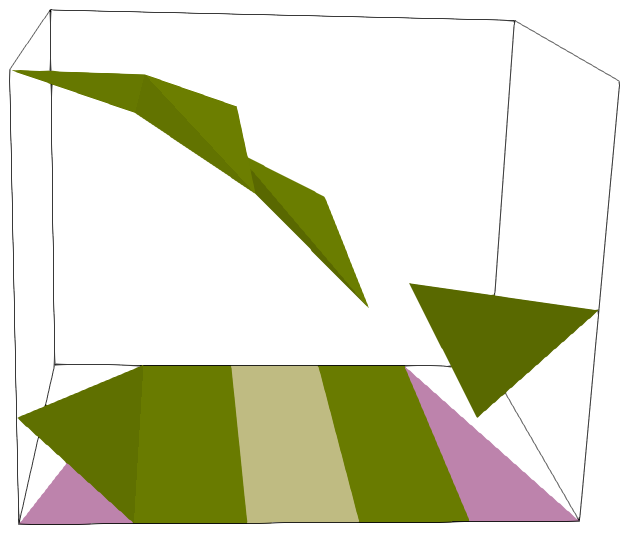
\includegraphics[width=0.8\linewidth]{top10nl_9x9_5_single}
\vspace{3mm} %for some reason, the space above the caption is not enough
\caption{The SSC of merging sequence~I, 
    shown in \fig\ref{fig:face_tgap}.}
\label{fig:ssc_single}
}
%\hfill
\parbox{.49\linewidth}{
\centering
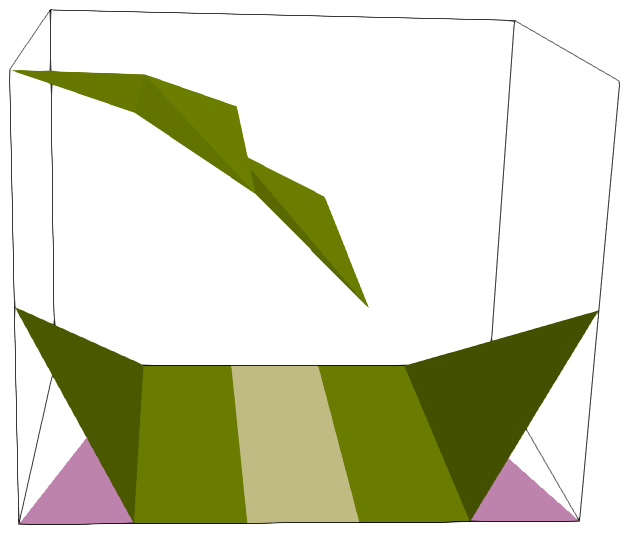
\includegraphics[width=0.8\linewidth]{top10nl_9x9_5_parallel}
\vspace{3mm} %for some reason, the space above the caption is not enough
\caption{The SSC of merging sequence~II, 
    shown in \fig\ref{fig:face_tgap}.}
\label{fig:ssc_parallel}
}
\end{figure}




\subsection{Snapping to an Existing State}
\label{sec:snap}

For a zooming action
(that is, slicing the SSC with a horizontal plane), 
we always snap the map to an existing state
so that users will not see a merging operation stops half-way
and will not see transition artifact (such as slivers or blended colors).
Take \fig\ref{fig:smooth_merging} for example, 
the merging animation should stop at 
either \ref{fig:smooth_merging}a or \ref{fig:smooth_merging}e,
but not at \ref{fig:smooth_merging}b, \ref{fig:smooth_merging}c, 
or \ref{fig:smooth_merging}d.
Moreover, some states do not exist because of the parallel events.
Such a case can be found in sequence~II of \fig\ref{fig:face_tgap},
where state~$1$ does not exist.
In this case, the merging animation should not stop at state~$1$.
In order to snap to existing state, 
we compress the information of merging events into 
a JSON file (JavaScript Object Notation File).
Then, the JSON file will be sent to the client side and uncompressed.


\subsubsection{On the Server Side}
\label{sec:snap_server}

On the server side, we compute the values shown in \tbl\ref{tbl:sequence_greedy}.
\tbl\ref{tbl:sequence_greedy} is based on the merging steps of
\fig\ref{fig:sequence_greedy},
where parallel parameter~$r_\mathrm{parallel} = 0.3$ is used.
The computation starts from step~$1$.
At the beginning, there are $7$ areas on the map, \ie$M_0$.
According to \eq\ref{eq:n_expect},
we expect to parallel three events ($n_{\mathrm{expect},1} = 3$).
However, only two event can be paralleled at step~$1$ of
\fig\ref{fig:sequence_greedy}.
Therefore, we have~$n_{\mathrm{event},1} = 2$.
Then, the difference of the expected value and the real value
can be computed by
\begin{equation}
\label{eq:n_diff}
n_{\mathrm{diff},i} = n_{\mathrm{expect},i} - n_{\mathrm{event},i}.
\end{equation}
That is, we have~$n_{\mathrm{diff},1}=1$ for step~$1$
(also see the $n_\mathrm{diff}$ value in the first row of \tbl\ref{tbl:sequence_greedy}).
We require that the starting state is~$s_{\mathrm{start},1} = 0$ for the first step.
Then, the ending state can be computed by
\begin{equation}
\label{eq:state_end}
s_{\mathrm{end},i} = s_{\mathrm{start},i} + n_{\mathrm{event},i}.
\end{equation}
That is, we have~$s_{\mathrm{end},1}=2$
(also see the state\_end value in the first row of \tbl\ref{tbl:sequence_greedy}).
At this point, the computation for step~$1$ completes.


\begin{figure}[tb]
%\centering
%\includegraphics[page=2]{blocked_polygons}
%\caption{.
%}
%\label{fig:sequence_greedy}
%\vspace{6mm} %for some reason, the space below the caption is not enough
%
%
%
\captionsetup*{type=table} %*: suppress warning "The caption type was already set to figure"
\caption{Some information of the merging sequence shown in \tbl\ref{tbl:sequence_greedy}.
Column~$n_\mathrm{area}$ shows the area number of the map at starting state~$s$,
that is, $|M_s|$ of \eq\ref{eq:n_expect}.
}
\label{tbl:sequence_greedy}
\centering
\begin{tabular}{ccccccc}
	\hline
	step & $n_\mathrm{area}$ & $n_\mathrm{expect}$ 
	& $n_\mathrm{event}$ & $n_\mathrm{diff}$ & state\_start & state\_end \\ \hline
	1        & 7      & 3        & 2        & 1     & 0      & 2      \\
	2        & 5      & 2        & 1        & 1     & 2      & 3      \\
	3        & 4      & 2        & 1        & 1     & 3      & 4      \\
	4        & 3      & 1        & 1        & 0     & 4      & 5      \\
	5        & 2      & 1        & 1        & 0     & 5      & 6      \\ \hline
%	6     & 1      & ---      & ---      & ---    \\ \hline
\end{tabular}
\end{figure}

For the next step, the number of areas can be computed by
$$
n_{\mathrm{area},i+1} = n_{\mathrm{area},i} - n_{\mathrm{event},i},
$$
where variable~$n_{\mathrm{area},i}$ denotes the area number 
at the starting state of step~$i$.
Furthermore, the starting state, $s_{\mathrm{start},i+1}$, is the same as  
$s_{\mathrm{end},i}$.
Based on~$n_{\mathrm{area},i+1}$ and~$s_{\mathrm{start},i+1}$,
other values of this step can be computed.
This process starts from step~$i=1$ and ends until only one area left.
As a result, we have all the values of \tbl\ref{tbl:sequence_greedy}.


%Then the difference in step~$i$ is
%\begin{equation}
%\label{eq:n_diff}
%n_{\mathrm{diff},i} = n_{\mathrm{expect},i} - n_{\mathrm{event},i},
%\end{equation}
%where variables~$n_{\mathrm{expect},i}$ and~$n_{\mathrm{event},i}$
%are respectively the expected and the real numbers of events in step~$i$,
%which are consistent with the definitions of 
%\eqs\ref{eq:n_expect} and~\ref{eq:n_event_state}.
%For the next step, we compute
%$$
%n_{\mathrm{area},i+1} = n_{\mathrm{area},i} - n_{\mathrm{event},i},
%$$
%where variable~$n_{\mathrm{area},i}$
%represents the area number at the starting state of step~$i$.
%Based on number~$n_{\mathrm{area},i+1}$,
%we can further compute $n_{\mathrm{expect},i+1}$ and obtain $n_{\mathrm{event},i+1}$.
%This process starts from step~$i=1$ and ends until only one area left.

Now, we have a column of $n_\mathrm{diff}$ values.
We compress those values as the form of 
$$
[[n_{\mathrm{diff},1},j_1], [n_{\mathrm{diff},j_1},j_2], \ldots, 
[n_{\mathrm{diff},i},j_k], [n_{\mathrm{diff},i+j_k},j_{k+1}], \ldots],
$$
where variable~$j_k$ is the number of the same $n_\mathrm{diff}$ values in a row 
starting at step~$i$.
Take the values of \tbl\ref{tbl:sequence_greedy} for example, 
$j_0$ is~$3$ 
because the first three~$n_\mathrm{diff}$ values are the same (\ie1),
and $j_1$ is~$2$ 
because the following two~$n_\mathrm{diff}$ values are the same (\ie0). 
According to our strategy, 
the $n_\mathrm{diff}$ values of \tbl\ref{tbl:sequence_greedy}
will be compressed to $[[1,3], [0,2]]$,
where each pair of values in the inner square brackets 
represent the event number and the repeat times.
The content of the JSON file is as following.
\begin{verbatim}
                {
                    "face_num": 7,
                    "parallel_param": 0.3,                    
                    "eventdiff_repetition": [[1, 3], [0, 2]]
                }
\end{verbatim}
If we would have a list of $n_\mathrm{diff}$ values~$[0, 0, 0, 0, 0, 0, 5, 0, 0]$,
then the compressed content would be~$[[0,6], [5,1], [0,2]]$.
Our case study will show that this way of compressing is efficient
(see \sect\ref{sec:case_study}).



\subsubsection{On the Client Side}
\label{sec:snap_client}


When a user opens our web map,
the JSON file will be sent to the client side.
We can unpack the content of entry ``eventdiff\_repetition'' and 
get the list of $n_\mathrm{diff}$ values~$[1, 1, 1, 0, 0]$.
Starting from step~$i=1$,
we can again compute~$n_{\mathrm{expect},i}$ according to \eq\ref{eq:n_expect},
where parallel parameter~$r_\mathrm{parallel}=0.3$ 
and face number~$n_{\mathrm{area},1} = 7$
can be obtained also from the JSON file.
Then, we can computer the actual number of parallel events by
\begin{equation*}
\label{eq:n_event_step}
n_{\mathrm{event},i} = n_{\mathrm{expect},i} - n_{\mathrm{diff},i},
\end{equation*}
which is an inverse function of \eq\ref{eq:n_diff}.
The computed~$n_\mathrm{event}$ values 
should be the same as the values before compressing
(see column~$n_\mathrm{event}$ in \tbl\ref{tbl:sequence_greedy}).

According to the~$n_\mathrm{event}$ values,
we can compute the accumulated number of events~$L_\mathrm{event} = 
[0, 2, 3, 4, 5, 6]$,
which is also the list of existing states
(see columns~state\_start and state\_end in \tbl\ref{tbl:sequence_greedy}).
According to how much a user has zoomed,
a scale, say $1:S_t$, can be computed.
According to \citet{Huang2016Webmap},
the number of merging events that should be processed can be computed by
\begin{equation}
\label{eq:E_t}
E_t = N_b \left(1-\frac{S^2_b}{S^2_t}\right),
\end{equation}
where parameter~$S_b$ is the scale denominator of the base map,
and parameter~$N_b = |M_0|$ is the number of areas on the base map.
In our example regarding to list~$L_\mathrm{event}$,
if event number~$E_t \le 0$, the base map should be presented;
if $E_t \ge 6$, the last value of list~$L_\mathrm{event}$,
the map with all the merging events having been processed
should be presented.
Otherwise, if $0<E_t < 6$, we snap event number~$E_t$ 
to the closest value in list~$L_\mathrm{event}$,
which is marked by~$E_{t,\mathrm{snap}}$.
The scale denominator corresponding to event number~$E_{t,\mathrm{snap}}$
can be computed by 
\begin{equation}
\label{eq:S_t_snap}
S_{t,\mathrm{snap}} = S_b \sqrt{\frac{N_b}{N_b-E_{t,\mathrm{snap}}}}.
\end{equation}
Note that \eq\ref{eq:S_t_snap} is an inverse function of \eq\ref{eq:E_t}.
At the end of the zooming action, 
the map will snap to state~$E_{t,\mathrm{snap}}$,
which is at scale~$1:S_{t,\mathrm{snap}}$.


%\subsection{Line simplification (smoothly moving vertices for the SSC)}


\section{Case Study}
\label{sec:case_study}


The dataset used in this case study is a subset of TOP10NL\footnote{%
More information about TOP10NL can be found at
\url{https://zakelijk.kadaster.nl/-/topnl},
accessed: Jan 14, 2020.},
produced by Kadaster.
%
\figs\ref{fig:data}a and~\ref{fig:data}c show the map and the legend\footnote{%
More details about the type code and the rendering formula can be found at
\url{http://register.geostandaarden.nl/visualisatie/top10nl/1.2.0/BRT_TOP10NL_1.2_beschrijving_visualisatie.xlsx},
accessed: Jan 15, 2020.}.
%
Because the base scale is $1:10{,}000$, 
we have~$S_b = 10{,}000$ for \eq\ref{eq:S_t_snap}.
The maximum value of event number~$E_{t,\mathrm{snap}}$ is~$13{,}237$
as there are in total~$13{,}238$ areas.
When we zoom out far enough 
so that~$E_{t,\mathrm{snap}}$ reaches its maximum value,
the scale denominator will arrive at~$1{,}150{,}565$
according to \eq\ref{eq:S_t_snap}.
At that moment, all the areas are merged into one single area
(see \figs\ref{fig:data}b).
In each step, we want to parallelly merge some portion of the areas.
We tried three cases: 0.1\%, 1\%, and 10\%.
The three version of maps can be browsed online at\footnote{%
\url{http://}}
That is, parallel parameter~$r_\mathrm{parallel}=0.001, 0.01, \text{and~} 0.1$ 
(see \sect\ref{sec:greedy_algo}).
Some statistics of the results are shown in 
\tbl\ref{tbl:parallel_param_comparison}.

\begin{figure}[tb]
\centering
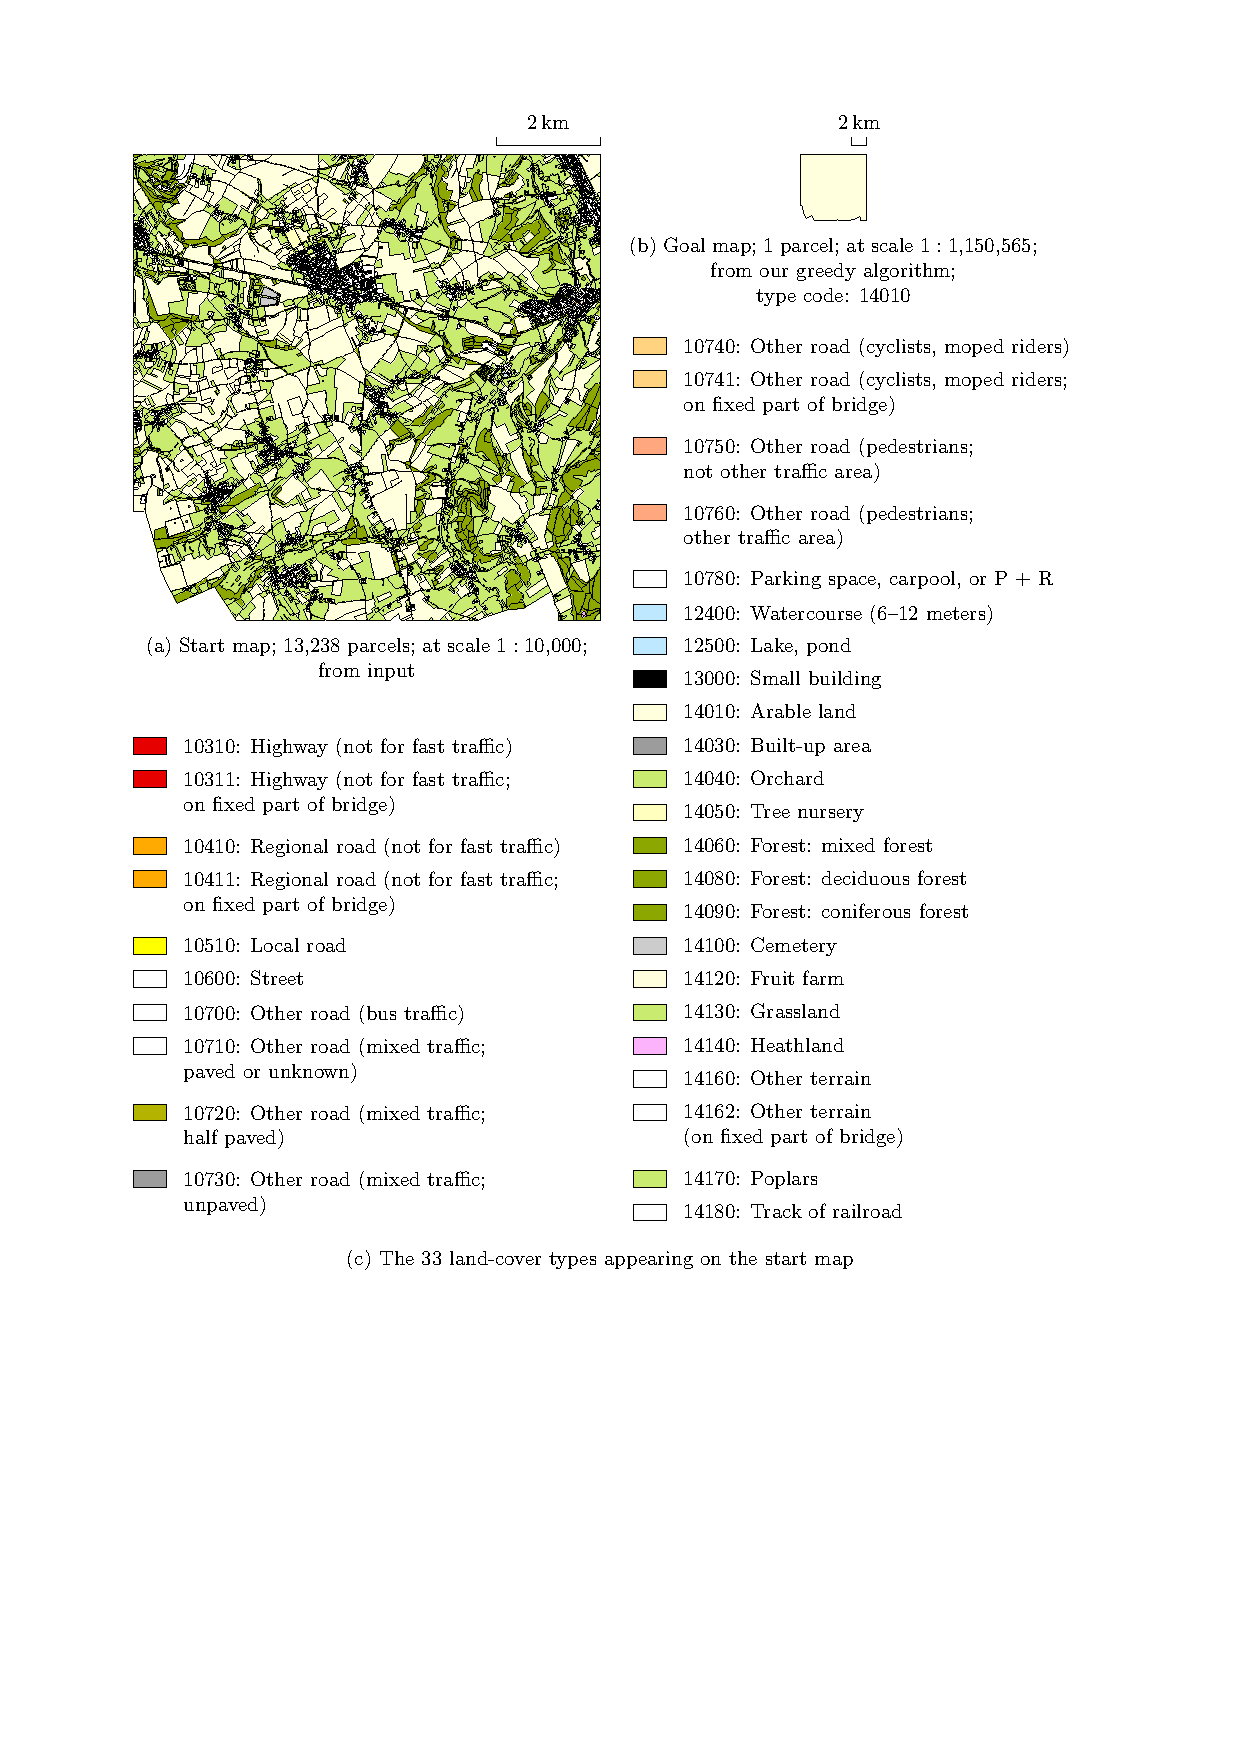
\includegraphics[page=1]{data}
\caption{The dataset represents the place 
    to the southeast of Maastricht, Limburg, The Netherlands.}
\label{fig:data}
\end{figure}


\begin{table}[tb]
\centering
\caption{pass}
\begin{tabular}{rrrr}
\hline
$r_\mathrm{parallel}$   & $L_\mathrm{diff\_rep}$        & $n_\mathrm{blocked}$  & $n_\mathrm{nbr\_blocked}$ \\ \hline
0.001                   & [[0, 3195]]                   &       228             &       72                  \\
0.01                    & [[0, 544]]                    &   3{,}216             &  1{,}841                  \\
0.1                     & $L_{\mathrm{diff\_rep}, 0.1}$ & 105{,}980             & 38{,}232                  \\ \hline 
\end{tabular}
%\begin{tabular}{cccc}
%\hline
%$r_\mathrm{parallel}$ & 0.001       & 0.01          & 0.1    \\ \hline
%eventdiff\_repetition & [[0, 3195]] & [[0, 544]]    & $L_{\mathrm{diff\_rep}, 0.1}$   \\
%least face blocked    & 228            & 3{,}216         & 105{,}980       \\
%best neighbor blocked & 72            & 1{,}841        & 38{,}232 \\ \hline 
%\end{tabular}
\begin{Verbatim}[fontfamily=normal,commandchars=\\\{\},
codes={\catcode`$=3\catcode`^=7\catcode`_=8}]
$L_{\mathrm{diff\_rep},0.1}$ = [[51, 1], [138, 1], [152, 1], [200, 1], [205, 1], [181, 1], [198, 1], [167, 1], [173, 1], [165, 1], 
[153, 1], [143, 1], [140, 1], [127, 1], [125, 1], [108, 1], [103, 1], [92, 2], [84, 1], [79, 1], [74, 1], [68, 1], 
[60, 1], [54, 1], [46, 1], [50, 1], [48, 1], [45, 1], [39, 1], [44, 1], [37, 1], [36, 1], [32, 1], [30, 1], [26, 1], 
[28, 1], [21, 2], [18, 1], [20, 1], [16, 1], [12, 1], [13, 1], [8, 1], [12, 2], [6, 1], [12, 1], [11, 1], [8, 1], [7, 1], 
[6, 1], [7, 1], [4, 1], [5, 1], [4, 1], [5, 2], [7, 1], [5, 1], [4, 1], [5, 1], [3, 1], [4, 1], [3, 3], [2, 2], [1, 2], [2, 1], 
[1, 2], [2, 1], [1, 3], [0, 2], [1, 2], [0, 14]]
\end{Verbatim}
%\fvset{gobble=2}
%\begin{Verbatim}[fontfamily=normal,frame=single,
%label=$L_{\mathrm{diff\_rep}, 0.1}$]
%   [[51, 1], [138, 1], [152, 1], [200, 1], [205, 1], [181, 1], [198, 1], [167, 1], [173, 1], [165, 1], 
%    [153, 1], [143, 1], [140, 1], [127, 1], [125, 1], [108, 1], [103, 1], [92, 2], [84, 1], [79, 1], [74, 1], [68, 1], 
%    [60, 1], [54, 1], [46, 1], [50, 1], [48, 1], [45, 1], [39, 1], [44, 1], [37, 1], [36, 1], [32, 1], [30, 1], [26, 1], 
%    [28, 1], [21, 2], [18, 1], [20, 1], [16, 1], [12, 1], [13, 1], [8, 1], [12, 2], [6, 1], [12, 1], [11, 1], [8, 1], [7, 1], 
%    [6, 1], [7, 1], [4, 1], [5, 1], [4, 1], [5, 2], [7, 1], [5, 1], [4, 1], [5, 1], [3, 1], [4, 1], [3, 3], [2, 2], [1, 2], [2, 1], 
%    [1, 2], [2, 1], [1, 3], [0, 2], [1, 2], [0, 14]]
%\end{Verbatim}
\label{tbl:parallel_param_comparison}
\end{table}

We have employed the ``Eater'' of \citet{Suba2014Merge},
implemented in Python, 
to generate the elements
(vertices, triangulated faces, and boundaries)
of the SSC \citep{vanOosterom2014tGAPSSC} 
and saved these elements in an OBJ file\footnote{%
Wavefront .obj file:
\url{https://en.wikipedia.org/wiki/Wavefront_.obj_file},
accessed: Jan 14, 2020.}.
%
The OBJ file and the JSON file (described in \sect\ref{sec:snap_server}) 
will be sent to the client 
when a user visits our website to access the map.
On the client side,
the two files are processed
by a prototype implemented in JavaScript.
The processed content and some code for WebGL (Web Graphics Library)
are submitted to GPU to display the map of smooth zoom.


In the following, we show some results for the case of 
parallel parameter~$r_\mathrm{parallel}= 0.01$.
The content of the JSON file is 
\begin{verbatim}
                {
                    "face_num": 13238,
                    "parallel_param": 0.01,                    
                    "eventdiff_repetition": [[0, 544]]
                }
\end{verbatim}
According to entry ``eventdiff\_repetition'',
there are~$544$ steps in total, 
which can be computed by summing up the second values 
of all the pairs of inner brackets.
There is only one pair of inner brackets when $r_\mathrm{parallel}= 0.01$,
but there are many pairs when $r_\mathrm{parallel}= 0.1$ 
(see $L_\mathrm{diff\_rep}$ in \tbl\ref{tbl:parallel_param_comparison}).
%
As explained in \sect\ref{sec:greedy_algo}, 
for each merging step we iteratively select the least important area 
and its most compatible neighbor to form a merging event; 
then, we block the neighbors of the two areas.
Sometimes, a least important area is already blocked 
because of the previously found events.
This situation happens~$3{,}216$ times in total for all the steps.
%
Sometimes, although a least important area is free, 
its most compatible neighbor has been blocked 
because of the previously found events.
This case happens~$1{,}841$ times in total for all the steps.
%










\section{Concluding Remarks}
\label{sec:concluding_remarks}

\subsection{Conclusion}
This paper proposed a greedy algorithm to find parallel events of 
merging land-cover areas.
Then, we integrated the parallel events into the SSC. 
On the client side, web maps are generated by slicing the SSC
based on the method of \citet{Meijers2020Web}.
To avoid half-way merging, we require the merging animation 
to stop at complete states (which contain parallel events).
Our case study shows that 
our approach provides with smoother transition for zooming.


\subsection{Future Work}



Our current event consists of only the merging operation,
it is also necessary to involve split operation
because sometimes a merging operation results in an unnatural area.
For example, it is weird to merge a long and thin area 
with one of the areas that are along it
\citep[see][]{Haunert2008Skeleton}.
Therefore, such kind of long and thin areas should be
split into several parts first.
We may integrate a split method based on the straight skeleton
\citep{Haunert2008Skeleton}
or the skeleton based on constrained Delaunay triangulation
\citep{Meijers2016Split}.
In order to apply appropriate generalization operators
for a certain scale,
we also need to extend and implement the framework 
to guide our generalization choices
\citep{Meijers2018Framework}.

To avoid clutter of vertices for zooming out, 
we also need to simplify the boundaries of the areas.
\citet{Meijers2011LineSimp} proposed a method 
to simplify the boundaries parallelly. 
Moreover, their results are topologically safe . 
Another choice would be the method of \citet{ImaiIri1988},
which is able to minimize the number of vertices 
for a given error threshold.
One more choice would be to construct compatible triangulations 
\citep[see][\chap3]{Peng2019Thesis}
for the two levels of land-cover maps.
In the SSC, we could build some tilted walls 
to connect the two levels of compatible triangulations.
When we slice this SSC to animate a zooming action,
the boundaries of the areas are morphed 
between a detailed representation and a coarse representation.
We can imagine that it is challenging to build the tilted walls.

evenly distribute the merging events for each step, 
network simplification

When we remove a triangle by slicing the SSC, 
we may want to keep three vertices of the triangle 
instead of making four vertices.
In this case, the polyhedron (with five faces) should have curly edges,
which is also known as a \emph{curved polyhedron}.
The slopes of curly edges need to be studied.

\fig\ref{fig:smooth_merging} shows our current solution of
gradually expanding an area over the other area.
In order to make the expansion even smoother,
we would like to implement the way 
shown in \fig\ref{fig:smooth_merging_future}.

\begin{figure}[tb]
\centering
\includegraphics[page=2]{smooth_merging}
\caption{A smooth way of merging two areas.
    The larger area expands over the smaller one.
    At the same time, 
    the smaller area gradually adapt to the color of the larger one,
    and the common boundary becomes thinner and thinner.}
\label{fig:smooth_merging_future}
\end{figure}

This paper used a greedy algorithm 
to find parallel merging events for each step.
Alternatively, it is also possible to find a sequence of merging steps,
where each step consists only one merging event, by some existing methods
(e.g., the greedy algorithm of \citet{vanOosterom2005}
or the \Astar algorithm of \citet[\chap2]{Peng2019Thesis}).
Then, we can reorganize some of the single-event merging steps 
to form some parallel-event merging steps.

This paper develops technique for smooth zooming based on parallel merging,
and we hope that it allows map users to follow the zooming more easily.
A future work is to investigate 
how much map users benefit from our technique.
We will conduct some usability tests based on the experience of
\citet[\sect6.7]{Suba2017Thesis} and \citet{Midtbo2007}.












































%Some research questions are as follows.
%What aspects should we optimize 
%(e.g., minimizing the number of merging events or 
%assigning similar numbers of merging steps to each event)?
%What algorithm should we use 
%(e.g., dynamic programming, \Astar, or integer linear programming)?
%How much time is gained for users to observe the merging steps on the screen?
%How to store the parallel merging steps?









%%%%%%%%%%%%%%%%%%%%%%%%%%%%%%%%%%%%%%%%%%%
%\section{Patents}
%This section is not mandatory, but may be added if there are patents resulting from the work reported in this manuscript.
%
%%%%%%%%%%%%%%%%%%%%%%%%%%%%%%%%%%%%%%%%%%%
%\vspace{6pt} 
%
%%%%%%%%%%%%%%%%%%%%%%%%%%%%%%%%%%%%%%%%%%%
%%% optional
%%\supplementary{The following are available online at \linksupplementary{s1}, Figure S1: title, Table S1: title, Video S1: title.}
%
%% Only for the journal Methods and Protocols:
%% If you wish to submit a video article, please do so with any other supplementary material.
%% \supplementary{The following are available at \linksupplementary{s1}, Figure S1: title, Table S1: title, Video S1: title. A supporting video article is available at doi: link.}
%
%%%%%%%%%%%%%%%%%%%%%%%%%%%%%%%%%%%%%%%%%%%
%\authorcontributions{For research articles with several authors, a short paragraph specifying their individual contributions must be provided. The following statements should be used ``conceptualization, X.X. and Y.Y.; methodology, X.X.; software, X.X.; validation, X.X., Y.Y. and Z.Z.; formal analysis, X.X.; investigation, X.X.; resources, X.X.; data curation, X.X.; writing--original draft preparation, X.X.; writing--review and editing, X.X.; visualization, X.X.; supervision, X.X.; project administration, X.X.; funding acquisition, Y.Y.'', please turn to the  \href{http://img.mdpi.org/data/contributor-role-instruction.pdf}{CRediT taxonomy} for the term explanation. Authorship must be limited to those who have contributed substantially to the work reported.}
%
%%%%%%%%%%%%%%%%%%%%%%%%%%%%%%%%%%%%%%%%%%%
%\funding{Please add: ``This research received no external funding'' or ``This research was funded by NAME OF FUNDER grant number XXX.'' and  and ``The APC was funded by XXX''. Check carefully that the details given are accurate and use the standard spelling of funding agency names at \url{https://search.crossref.org/funding}, any errors may affect your future funding.}
%
%%%%%%%%%%%%%%%%%%%%%%%%%%%%%%%%%%%%%%%%%%%
%\acknowledgments{In this section you can acknowledge any support given which is not covered by the author contribution or funding sections. This may include administrative and technical support, or donations in kind (e.g., materials used for experiments).}
%
%%%%%%%%%%%%%%%%%%%%%%%%%%%%%%%%%%%%%%%%%%%
%\conflictsofinterest{Declare conflicts of interest or state ``The authors declare no conflict of interest.'' Authors must identify and declare any personal circumstances or interest that may be perceived as inappropriately influencing the representation or interpretation of reported research results. Any role of the funders in the design of the study; in the collection, analyses or interpretation of data; in the writing of the manuscript, or in the decision to publish the results must be declared in this section. If there is no role, please state ``The funders had no role in the design of the study; in the collection, analyses, or interpretation of data; in the writing of the manuscript, or in the decision to publish the results''.} 
%
%%%%%%%%%%%%%%%%%%%%%%%%%%%%%%%%%%%%%%%%%%%
%%% optional
%\abbreviations{The following abbreviations are used in this manuscript:\\
%
%\noindent 
%\begin{tabular}{@{}ll}
%MDPI & Multidisciplinary Digital Publishing Institute\\
%DOAJ & Directory of open access journals\\
%TLA & Three letter acronym\\
%LD & linear dichroism
%\end{tabular}}
%
%%%%%%%%%%%%%%%%%%%%%%%%%%%%%%%%%%%%%%%%%%%
%%% optional
%\appendixtitles{no} %Leave argument "no" if all appendix headings stay EMPTY (then no dot is printed after "Appendix A"). If the appendix sections contain a heading then change the argument to "yes".
%\appendix
%\section{}
%\unskip
%\subsection{}
%The appendix is an optional section that can contain details and data supplemental to the main text. For example, explanations of experimental details that would disrupt the flow of the main text, but nonetheless remain crucial to understanding and reproducing the research shown; figures of replicates for experiments of which representative data is shown in the main text can be added here if brief, or as Supplementary data. Mathematical proofs of results not central to the paper can be added as an appendix.
%
%\section{}
%All appendix sections must be cited in the main text. In the appendixes, Figures, Tables, etc. should be labeled starting with `A', e.g., Figure A1, Figure A2, etc. 

%%%%%%%%%%%%%%%%%%%%%%%%%%%%%%%%%%%%%%%%%%
% Citations and References in Supplementary files are permitted provided that they also appear in the reference list here. 

%=====================================
% References, variant A: internal bibliography
%=====================================
%\reftitle{References}
%\begin{thebibliography}{999}
%% Reference 1
%\bibitem[Author1(year)]{ref-journal}
%Author1, T. The title of the cited article. {\em Journal Abbreviation} {\bf 2008}, {\em 10}, 142--149.
%% Reference 2
%\bibitem[Author2(year)]{ref-book}
%Author2, L. The title of the cited contribution. In {\em The Book Title}; Editor1, F., Editor2, A., Eds.; Publishing House: City, Country, 2007; pp. 32--58.
%\end{thebibliography}
\bibliography{Reference/BibReference}

% The following MDPI journals use author-date citation: Arts, Econometrics, Economies, Genealogy, Humanities, IJFS, JRFM, Laws, Religions, Risks, Social Sciences. For those journals, please follow the formatting guidelines on http://www.mdpi.com/authors/references
% To cite two works by the same author: \citeauthor{ref-journal-1a} (\citeyear{ref-journal-1a}, \citeyear{ref-journal-1b}). This produces: Whittaker (1967, 1975)
% To cite two works by the same author with specific pages: \citeauthor{ref-journal-3a} (\citeyear{ref-journal-3a}, p. 328; \citeyear{ref-journal-3b}, p.475). This produces: Wong (1999, p. 328; 2000, p. 475)

%=====================================
% References, variant B: external bibliography
%=====================================
%\externalbibliography{yes}
%\bibliography{your_external_BibTeX_file}

%%%%%%%%%%%%%%%%%%%%%%%%%%%%%%%%%%%%%%%%%%
%% optional
%\sampleavailability{Samples of the compounds ...... are available from the authors.}

%% for journal Sci
%\reviewreports{\\
%Reviewer 1 comments and authors’ response\\
%Reviewer 2 comments and authors’ response\\
%Reviewer 3 comments and authors’ response
%}




%%%%%%%%%%%%%%%%%%%%%%%%%%%%%%%%%%%%%%%%%%
\end{document}

